\documentclass{beamer}

\mode<presentation> {

% The Beamer class comes with a number of default slide themes
% which change the colors and layouts of slides. Below this is a list
% of all the themes, uncomment each in turn to see what they look like.

%\usetheme{default}
%\usetheme{AnnArbor}
%\usetheme{Antibes}
%\usetheme{Bergen}
%\usetheme{Berkeley}
%\usetheme{Berlin}
%\usetheme{Boadilla}
%\usetheme{CambridgeUS}
%\usetheme{Copenhagen}
%\usetheme{Darmstadt}
%\usetheme{Dresden}
%\usetheme{Frankfurt}
%\usetheme{Goettingen}
%\usetheme{Hannover}
%\usetheme{Ilmenau}
%\usetheme{JuanLesPins}
%\usetheme{Luebeck}
\usetheme{Madrid}
%\usetheme{Malmoe}
%\usetheme{Marburg}
%\usetheme{Montpellier}
%\usetheme{PaloAlto}
%\usetheme{Pittsburgh}
%\usetheme{Rochester}
%\usetheme{Singapore}
%\usetheme{Szeged}
%\usetheme{Warsaw}

% As well as themes, the Beamer class has a number of color themes
% for any slide theme. Uncomment each of these in turn to see how it
% changes the colors of your current slide theme.

%\usecolortheme{albatross}
%\usecolortheme{beaver}
%\usecolortheme{beetle}
%\usecolortheme{crane}
%\usecolortheme{dolphin}
%\usecolortheme{dove}
%\usecolortheme{fly}
%\usecolortheme{lily}
%\usecolortheme{orchid}
%\usecolortheme{rose}
%\usecolortheme{seagull}
%\usecolortheme{seahorse}
%\usecolortheme{whale}
%\usecolortheme{wolverine}

%\setbeamertemplate{footline} % To remove the footer line in all slides uncomment this line
%\setbeamertemplate{footline}[page number] % To replace the footer line in all slides with a simple slide count uncomment this line

%\setbeamertemplate{navigation symbols}{} % To remove the navigation symbols from the bottom of all slides uncomment this line
}

\usepackage[utf8]{inputenc}
\usepackage[english]{babel}
% \usepackage[ngerman]{babel}

\usepackage{mathtools}
\usepackage{amsmath}
\usepackage{amssymb}
\usepackage{amsfonts}
\usepackage{xcolor}
\usepackage{graphicx}
\usepackage{float}
\usepackage{algorithm}
\usepackage[noend]{algpseudocode}

\let\oldReturn\Return
\renewcommand{\Return}{\State\oldReturn}

\usepackage{tikz}
\usetikzlibrary{arrows,decorations.pathmorphing,positioning,decorations.markings,fit,trees,shapes,automata,shapes.multipart}
\usepackage{pgf-umlsd}
\usepgflibrary{arrows} % for pgf-umlsd

\tikzset{onslide/.code args={<#1>#2}{%
  \only<#1>{\pgfkeysalso{#2}} % \pgfkeysalso doesn't change the path
}}

\usepackage{listings}

\newcommand{\location}{\ell}
\newcommand{\valuation}{\sigma}
\newcommand{\Valuation}{\Sigma}
\newcommand{\update}{\eta}
\newcommand{\atom}{a}
\newcommand{\guard}{\tau}
\newcommand{\cost}{c}
\newcommand{\complexity}{\emph{complexity}}
\newcommand{\landau}{\mathcal{O}}
\newcommand{\constant}{\emph{constant}}

\newcommand{\ValueSet}{\bar{\mathbb{Z}}}

\newcommand{\abs}[1]{\left|#1\right|}

\newcommand{\LSize}{{\mathcal{S}^\sqcup}}
\newcommand{\USize}{{\mathcal{S}^\sqcap}}
\newcommand{\GSize}{{\mathcal{S}^\square}}
\newcommand{\Size}{{(\LSize, \USize)}}
\newcommand{\UTime}{{\mathcal{R}^\sqcap}}
\newcommand{\UCost}{{\mathcal{C}^\sqcap}}
\newcommand{\LLSB}{{\mathcal{S}^\sqcup_l}}
\newcommand{\ULSB}{{\mathcal{S}^\sqcap_l}}
\newcommand{\GLSB}{{\mathcal{S}^\square_l}}
\newcommand{\LSB}{{(\LLSB, \ULSB)}}

\newcommand{\dpre}[1]{{\tilde{d}^{#1}}}
\newcommand{\pret}{r}
\newcommand{\actt}{s}
\newcommand{\prerv}{\gamma}
\newcommand{\actrv}{\alpha}
\newcommand{\outrv}{\beta}
\newcommand{\prestate}{{\tilde{\valuation}}}
\newcommand{\actstate}{\valuation}
\newcommand{\ustate}{{\valuation^\sqcap}}
\newcommand{\lstate}{{\valuation^\sqcup}}
\newcommand{\prel}{{\tilde{\location}}}
\newcommand{\actl}{\location}

\newcommand{\scale}{\emph{scale}}
\newcommand{\incoming}{\emph{in}}
\newcommand{\start}{\emph{start}}
\newcommand{\sign}{\emph{sign}}
\newcommand{\effect}{\emph{effect}}
\newcommand{\SCC}{C}
\newcommand{\timerank}{\emph{timerank}}
\newcommand{\costrank}{\emph{costrank}}
\newcommand{\rv}{\alpha}
\newcommand{\RV}{\text{RV}}
\newcommand{\BoundSet}{\mathcal{B}}
\newcommand{\Program}{\mathcal{P}}
\newcommand{\AtomSet}{\mathcal{A}}
\newcommand{\ConstraintSet}{\mathcal{C}}
\newcommand{\TSet}{\mathcal{T}}
\newcommand{\tvar}{\lambda}
\newcommand{\VSet}{\mathcal{V}}
\newcommand{\TVSet}{\mathcal{TV}}
\newcommand{\PVSet}{\mathcal{PV}}
\newcommand{\AllVarsSet}{(\PVSet \cup \TVSet)}
\newcommand{\LSet}{\mathcal{L}}
\newcommand{\ScaledSum}{\dot{x}}
\newcommand{\pre}{\emph{pre}}
\newcommand{\actV}{\emph{actV}}
\newcommand{\maxO}[1]{\left\langle #1 \right\rangle}
\newcommand{\maximum}[1]{\max \left\lbrace #1 \right\rbrace}
\newcommand{\minimum}[1]{\min \left\lbrace #1 \right\rbrace}
\newcommand{\braced}[1]{\lbrace #1 \rbrace}

\newcommand{\usub}{\delta^\sqcap}
\newcommand{\lsub}{\delta^\sqcup}

\newcommand{\usubst}[3]{\left\lceil #1 \right\rceil^{#3}_{#2}}
\newcommand{\lsubst}[3]{\left\lfloor #1 \right\rfloor^{#3}_{#2}}

\newcommand{\exacteval}[2]{\left\llbracket #1 \right\rrbracket_{#2}}
\newcommand{\ueval}[3]{\left\lceil #1 \right\rceil^{#3}_{#2}}
\newcommand{\leval}[3]{\left\lfloor #1 \right\rfloor^{#3}_{#2}}

\newcommand{\timecomplexityterm}{
  \sup \braced{ k \in \mathbb{N} \mid \exists \valuation_0, (\location, \valuation): \lstate \leq \valuation_0 \leq \ustate \wedge (\location_0, \valuation_0) \rightarrow^k (\location, \valuation) }
}

\newcommand{\timeboundterm}{
  \sup \braced{ k \in \mathbb{N} \mid \exists \valuation_0, (\location, \valuation): \lstate \leq \valuation_0 \leq \ustate \wedge (\location_0, \valuation_0) (\rightarrow^* \circ \rightarrow_t)^k (\location, \valuation) }
}

\newcommand{\sizeboundterm}{
  \braced{ \valuation(v) \mid \exists \valuation_0, (\location, \valuation): \lstate \leq \valuation_0 \leq \ustate \wedge (\location_0, \valuation_0) (\rightarrow^* \circ \rightarrow_\actt) (\location, \valuation)}
}

\newcommand{\usizeboundterm}{\sup \sizeboundterm}
\newcommand{\lsizeboundterm}{\inf \sizeboundterm}

\newcommand{\localsizeboundterm}{
  \braced{\valuation'(v) \mid \exists (\location, \valuation), (\location', \valuation'): \lstate \leq \valuation \leq \ustate \wedge (\location, \valuation) \rightarrow_t (\location', \valuation')}
}

\newcommand{\ulocalsizeboundterm}{\sup \localsizeboundterm}
\newcommand{\llocalsizeboundterm}{\inf \localsizeboundterm}

\newcommand{\costcomplexityterm}{
  \braced{ \sum_{0 \leq i \leq k} \exacteval{\cost(t_i)}{\valuation_i} \mid \exists \valuation_0, k \geq 1: 
    \lstate \leq \valuation_0 \leq \ustate \wedge (\location_0, \valuation_0) \rightarrow_{t_0} (\location_1, \valuation_1) \rightarrow_{t_1} \dots \rightarrow_{t_k} (\location_k, \valuation_k) }
}

\newcommand{\Proof}[2]{
  \input{proofs/#2}
}


%----------------------------------------------------------------------------------------
%	TITLE PAGE
%----------------------------------------------------------------------------------------

\title[Non-Monotonic Bounds for Complexity Analysis of Integer Programs]{Non-Monotonic Bounds for Complexity Analysis of Integer Programs}
% The short title appears at the bottom of every slide, the full title is only on the title page

\author{Fabian B\"{o}ller} % Your name
\institute[i2] % Your institution as it will appear on the bottom of every slide, may be shorthand to save space
{
RWTH Aachen \\ % Your institution for the title page
\medskip
\textit{fabian.boeller@rwth-aachen.de} % Your email address
}
\date{WS 2017/18} % Date, can be changed to a custom date

\tikzset{
  transition/.style={align=left,draw},
  location/.style={circle,draw,font=\sffamily\bfseries},
  transitions/.style={
    every edge/.style={transition},
    every node/.style={font=\sffamily\small}
  },
  program/.style={
    ->,>=stealth',auto,node distance=3cm,thick,
    every node/.style={location}
  },  
  evaluation/.style={
    ->,>=stealth',auto,node distance=2cm,
    every text node part/.style={align=center},thick,
    every node/.style={draw,rectangle}
  },
  cross/.style={
    decoration={ markings,
      mark=at position .5 with {\draw[-,thick] (-2mm,2mm) -- (2mm,-2mm)node[inner sep=1pt,pos=0.5,auto]{#1};}  %% adjust 2mm etc as you wish
    },
    postaction={decorate}
  }
}
\begin{document}

\begin{frame}
\titlepage % Print the title page as the first slide
\end{frame}

\begin{frame}
\frametitle{Overview} % Table of contents slide, comment this block out to remove it
\tableofcontents % Throughout your presentation, if you choose to use \section{} and \subsection{} commands, these will automatically be printed on this slide as an overview of your presentation
\end{frame}

%----------------------------------------------------------------------------------------
%	PRESENTATION SLIDES
%----------------------------------------------------------------------------------------

\section{Introduction}

\begin{frame}
  \frametitle{Motivation}
  \begin{block}{Example program}
    \begin{algorithmic}
      \While{$x > y$}
        \State $x := x - 1$
      \EndWhile
    \end{algorithmic}
  \end{block}
  \begin{block}{Results}
    Actually: Program has $\maximum{0,x-y}$ steps \\
    Old: Program has maximum $\abs{x}+\abs{y}$ steps
  \end{block}
\end{frame}

\begin{frame}
  \frametitle{Programs}
  \begin{columns}
    \begin{column}{0.3\textwidth}
      \begin{algorithmic}
        \While{$x > y$}
        \State $x := x - 1$
        \EndWhile
      \end{algorithmic}
    \end{column}
    \begin{column}{0.5\textwidth}
      \begin{figure}
        \centering
        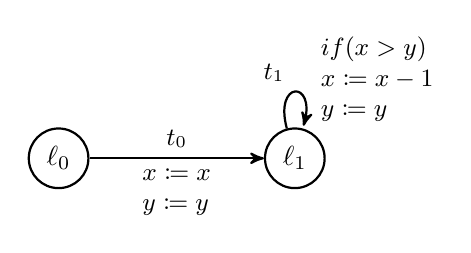
\begin{tikzpicture}[program]
          \node (0) {$\location_0$};
          \node (1) [right of=0] {$\location_1$};
          \path[transitions]
          (0) edge node[above] {$t_0$} node[below] {$x \coloneqq x$\\$y \coloneqq y$} (1)
          (1) edge[loop above] node[above left] {$t_1$} node[above right=-0.5cm and 0.2cm] {$if(x>y)$\\$x \coloneqq x-1$\\$y \coloneqq y$} (1)
          ;
        \end{tikzpicture}
      \end{figure}
    \end{column}
  \end{columns}
\end{frame}

\begin{frame}
  \frametitle{Time Complexity}
  \begin{figure}
    \centering
    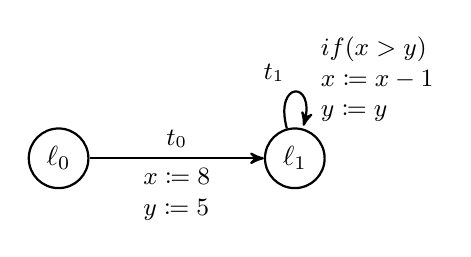
\begin{tikzpicture}[program]
      \node (0) {$\location_0$};
      \node (1) [right of=0] {$\location_1$};
      \path[transitions]
      (0) edge node[above] {$t_0$} node[below] {$x \coloneqq 8$\\$y \coloneqq 5$} (1)
      (1) edge[loop above] node[above left] {$t_1$} node[above right=-0.5cm and 0.2cm] {$if(x>y)$\\$x \coloneqq x-1$\\$y \coloneqq y$} (1)
      ;
    \end{tikzpicture}
  \end{figure}
  \begin{figure}
    \centering
    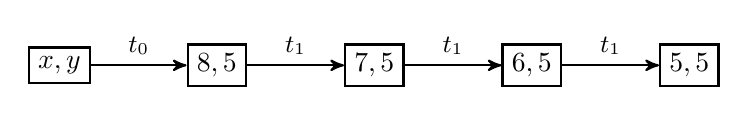
\begin{tikzpicture}[evaluation]
      
      \node (0) {$x,y$};
      \node (1) [right of=0] {$8,5$};
      \node (2) [right of=1] {$7,5$};
      \node (3) [right of=2] {$6,5$};
      \node (4) [right of=3] {$5,5$};
      
      \path[transitions]
      (0) edge node {$t_0$} (1)
      (1) edge node {$t_1$} (2)
      (2) edge node {$t_1$} (3)
      (3) edge node {$t_1$} (4)
      ;
    \end{tikzpicture}
  \end{figure}
  \begin{figure}
    \centering
    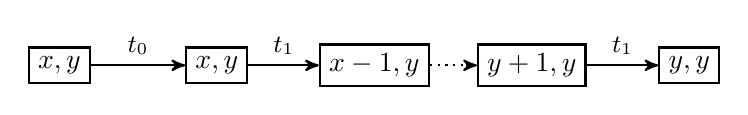
\begin{tikzpicture}[evaluation]
      
      \node (0) {$x,y$};
      \node (1) [right of=0] {$x,y$};
      \node (2) [right of=1] {$x-1,y$};
      \node (3) [right of=2] {$y+1,y$};
      \node (4) [right of=3] {$y,y$};
      
      \path[transitions]
      (0) edge node {$t_0$} (1)
      (1) edge node {$t_1$} (2)
      (2) edge[dotted] (3)
      (3) edge node {$t_1$} (4)
      ;
    \end{tikzpicture}
  \end{figure}
  \begin{block}{TODO}
    Mark 8 and 5 \\
    Animate
  \end{block}
\end{frame}

\begin{frame}
  \frametitle{Ranking Functions}
  \begin{figure}
    \centering
    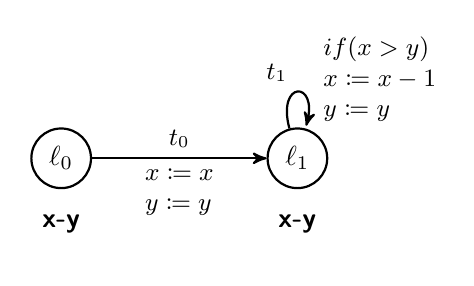
\begin{tikzpicture}[program]
      \node[label=below:{x-y}] (0) {$\location_0$};
      \node[label=below:{x-y}] (1) [right of=0] {$\location_1$};
      \path[transitions]
      (0) edge node[above] {$t_0$} node[below] {$x \coloneqq x$\\$y \coloneqq y$} (1)
      (1) edge[loop above] node[above left] {$t_1$} node[above right=-0.5cm and 0.2cm] {$if(x>y)$\\$x \coloneqq x-1$\\$y \coloneqq y$} (1)
      ;
    \end{tikzpicture}
  \end{figure}
  \begin{figure}
    \centering
    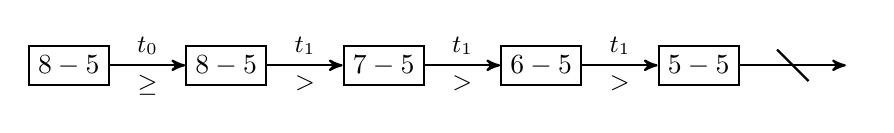
\begin{tikzpicture}[evaluation]
      
      \node (0) {$8-5$};
      \node (1) [right of=0] {$8-5$};
      \node (2) [right of=1] {$7-5$};
      \node (3) [right of=2] {$6-5$};
      \node (4) [right of=3] {$5-5$};
      \node (exit) [right of=4,draw=none] {};
      
      \path[transitions]
      (0) edge node {$t_0$} node[below] {$\geq$} (1)
      (1) edge node {$t_1$} node[below] {$>$} (2)
      (2) edge node {$t_1$} node[below] {$>$} (3)
      (3) edge node {$t_1$} node[below] {$>$} (4)
      (4) edge[cross] node[below] {} (exit)
      ;
    \end{tikzpicture}
  \end{figure}
  \begin{figure}
    \centering
    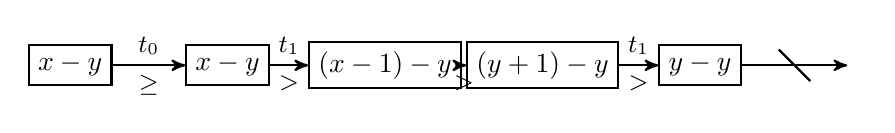
\begin{tikzpicture}[evaluation]
      
      \node (0) {$x-y$};
      \node (1) [right of=0] {$x-y$};
      \node (2) [right of=1] {$(x-1)-y$};
      \node (3) [right of=2] {$(y+1)-y$};
      \node (4) [right of=3] {$y-y$};
      \node (exit) [right of=4,draw=none] {};
      
      \path[transitions]
      (0) edge node {$t_0$} node[below] {$\geq$} (1)
      (1) edge node {$t_1$} node[below] {$>$} (2)
      (2) edge[dotted] node[below] {$>$} (3)
      (3) edge node {$t_1$} node[below] {$>$} (4)
      (4) edge[cross] node[below] {} (exit)
      ;
    \end{tikzpicture}
  \end{figure}
  \begin{block}{TODO}
  \end{block}
\end{frame}

\begin{frame}
  \frametitle{Time Bounds}
  \begin{figure}
    \centering
    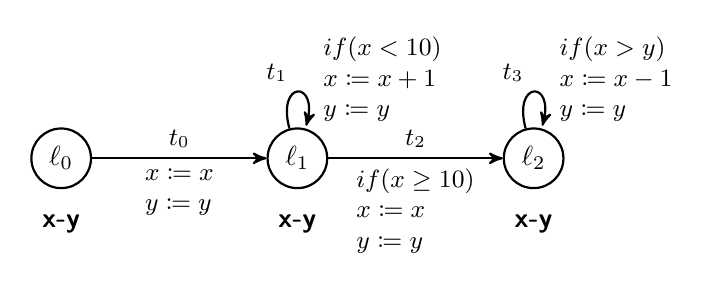
\begin{tikzpicture}[program]
      \node[label=below:{x-y}] (0) {$\location_0$};
      \node[label=below:{x-y}] (1) [right of=0] {$\location_1$};
      \node[label=below:{x-y}] (2) [right of=1] {$\location_2$};
      \path[transitions]
      (0) edge node[above] {$t_0$} node[below] {$x \coloneqq x$\\$y \coloneqq y$} (1)
      (1) edge[loop above] node[above left] {$t_1$} node[above right=-0.5cm and 0.2cm] {$if(x<10)$\\$x \coloneqq x+1$\\$y \coloneqq y$} (1)
      (1) edge node[above] {$t_2$} node[below] {$if(x \geq 10)$\\$x \coloneqq x$\\$y \coloneqq y$} (2)
      (2) edge[loop above] node[above left] {$t_3$} node[above right=-0.5cm and 0.2cm] {$if(x>y)$\\$x \coloneqq x-1$\\$y \coloneqq y$} (2)
      ;
    \end{tikzpicture}
  \end{figure}
  \begin{block}{Equation}
    $\UTime(t_0)$ \\
    $\UTime(t_0) \cdot (x-y)$ \\
    $\UTime(t_0) \cdot (\USize(t_0,x)-\LSize(t_0,y))$ \\
    $\UTime(t_0) \cdot (\USize(t_0,x)-\LSize(t_0,y)) + \UTime(t_1) \cdot (\USize(t_1,x)-\LSize(t_1,y))$ \\
    $\UTime(t_0) \cdot (\mathcal{S}(t_0,x)+\mathcal{S}(t_0,y)) + \UTime(t_1) \cdot (\mathcal{S}(t_1,x)+\mathcal{S}(t_1,y))$
  \end{block}
  \begin{block}{TODO}
    Show that $x-y$ is increasing with $t_2$ \\
    Show that it is still fine for $t_3$ and $t_4$ \\
    Explain need for size bounds
  \end{block}
\end{frame}

\begin{frame}
  \frametitle{Size Complexity}
  \begin{figure}
    \centering
    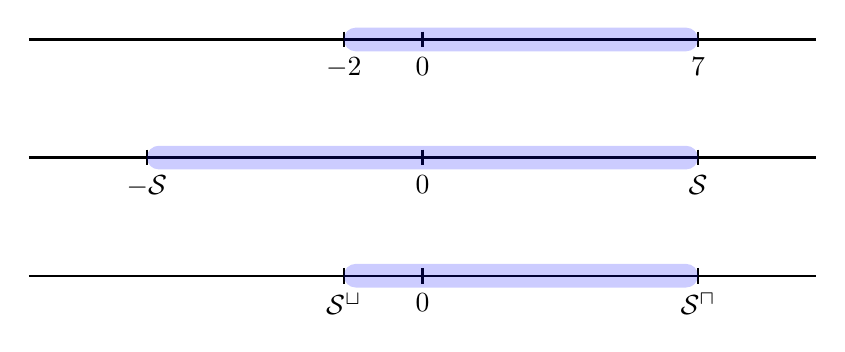
\begin{tikzpicture}[scale=0.5]
      \foreach \y/\lvalue/\uvalue/\llabel/\ulabel in {
        6/-2/7/$-2$/$7$,
        3/-7/7/$-\mathcal{S}$/$\mathcal{S}$,
        0/-2/7/$\LSize$/$\USize$
      } {
        \draw[-, thick] (-10,\y) -- (10,\y);
        \draw[thick] (0,\y+0.2) -- (0,\y-0.2) node[below] {0};
        \draw[thick] (\lvalue,\y+0.2) -- (\lvalue,\y-0.2) node[below] {\llabel};
        \draw[thick] (\uvalue,\y+0.2) -- (\uvalue,\y-0.2) node[below] {\ulabel};
        \fill[opacity=0.2,blue,rounded corners=1ex] (\lvalue,\y-0.3) -- (\uvalue,\y-0.3) -- (\uvalue,\y+0.3) -- (\lvalue,\y+0.3) -- cycle;
      }
    \end{tikzpicture}
  \end{figure}
\end{frame}

\begin{frame}
  \frametitle{Size Complexity}
  \begin{block}{Assignment}
    $x' \coloneqq x$
  \end{block}
  \begin{figure}
    \centering
    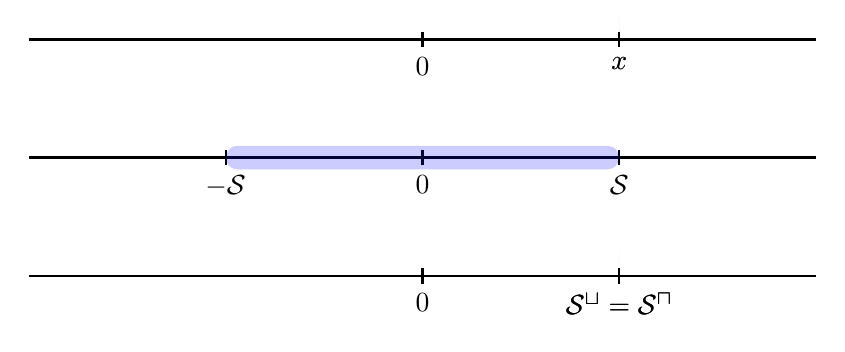
\begin{tikzpicture}[scale=0.5]
      \foreach \y/\lvalue/\uvalue/\llabel/\ulabel in {
        6/5/5/$x$/$x$,
        3/-5/5/$-\mathcal{S}$/$\mathcal{S}$,
        0/5/5/$\LSize=\USize$
      } {
        \draw[-, thick] (-10,\y) -- (10,\y);
        \draw[thick] (0,\y+0.2) -- (0,\y-0.2) node[below] {0};
        \draw[thick] (\lvalue,\y+0.2) -- (\lvalue,\y-0.2) node[below] {\llabel};
        \draw[thick] (\uvalue,\y+0.2) -- (\uvalue,\y-0.2) node[below] {\ulabel};
        \fill[opacity=0.2,blue,rounded corners=1ex] (\lvalue,\y-0.3) -- (\uvalue,\y-0.3) -- (\uvalue,\y+0.3) -- (\lvalue,\y+0.3) -- cycle;
      }
    \end{tikzpicture}
  \end{figure}
\end{frame}

\begin{frame}
  \frametitle{Size Complexity}
  \begin{block}{TODO}
    Define size complexity \\
    Example of size to $\location_0$
  \end{block}
\end{frame}

\begin{frame}
  \frametitle{Size Complexity}
  Explain difference between lower and upper and old size complexity
\end{frame}

\begin{frame}
  \frametitle{Local Size Bounds}
  Define local size bounds
\end{frame}

\begin{frame}
  \frametitle{Time Bounds}
  Back to the example
\end{frame}

\begin{frame}
  \frametitle{Size Bounds}
  Explain the advantages of good size bounds
  Present the three size bound examples from the thesis unrelated to the initial example
\end{frame}

\begin{frame}
  \frametitle{Size Bounds Caveat}
  Explain size bounds caveat of negating SCCs
\end{frame}

\section{Cost Bounds}

\begin{frame}
  \frametitle{Cost Complexity}
  \begin{block}{Time Complexity}
    TODO Recap
  \end{block}
  \pause
  \begin{block}{Size Complexity}
    TODO Recap
  \end{block}
  \pause
  \begin{block}{Cost Complexity}
    Explain with a call to a function $f$ in the initial example 
  \end{block}
\end{frame}

\begin{frame}
  \frametitle{Cost Complexity}
  Present the trivial approach of multiplying with the time bounds
\end{frame}

\begin{frame}
  \frametitle{Cost Ranking}
\end{frame}

\section{Conclusion}

\begin{frame}
  \frametitle{Conclusion}
\end{frame}

\end{document} 
